\chapter{Results}
\label{chap:results}

\section{Performance Evaluation}

\section{Ablation Studies}
\label{sec:ablation_studies}

\subsection{Question Module Ablations}
\label{subsec:question_module_ablations}

\subsection{Scene Graph Module Ablations}
\label{subsec:scene_graph_module_ablations}

{\color{red}TODO: GloVe only for scene graph and questions}

{\color{red}TODO: Ablations on scene graph embedding for best model only:
\begin{itemize}
    \item Removal of skip-edges in the graph
    \item Removal of relation data, with edges only occurring between objects where a relation would usually be (i.e. skip edges w/ no relation nodes)
    \item If time, removal of relation and attribute data as well.
\end{itemize}}

\begin{itemize}
    \item Includes more important initial tests, move less important ones to appendix.
\end{itemize}

\begin{itemize}
    \item GloVe vs random normal distribution. Glove required less tuning since the vector norms already worked well.
\end{itemize}

\section{Hyperparameter Optimisation}
\label{sec:hyperparameter_optimisation}

These results represent a total of 55 days of GPU compute

{\color{red}
  \begin{itemize}
    \item wandb \cite{wandb} implementation of bayesian optimisation, using the hyperband early stopping method
  \end{itemize}
}

The effects of the Hyperband method are clearly seen in \figureautorefname{ \ref{fig:hyperparameter_optimisation_validation_loss_and_accuracy}}, where only a few models are trained to completion and less promising models are stopped earlier to encourage exploration of the hyperparameter search space.

\begin{figure}
    \centering
    \begin{subfigure}[t]{\textwidth}
        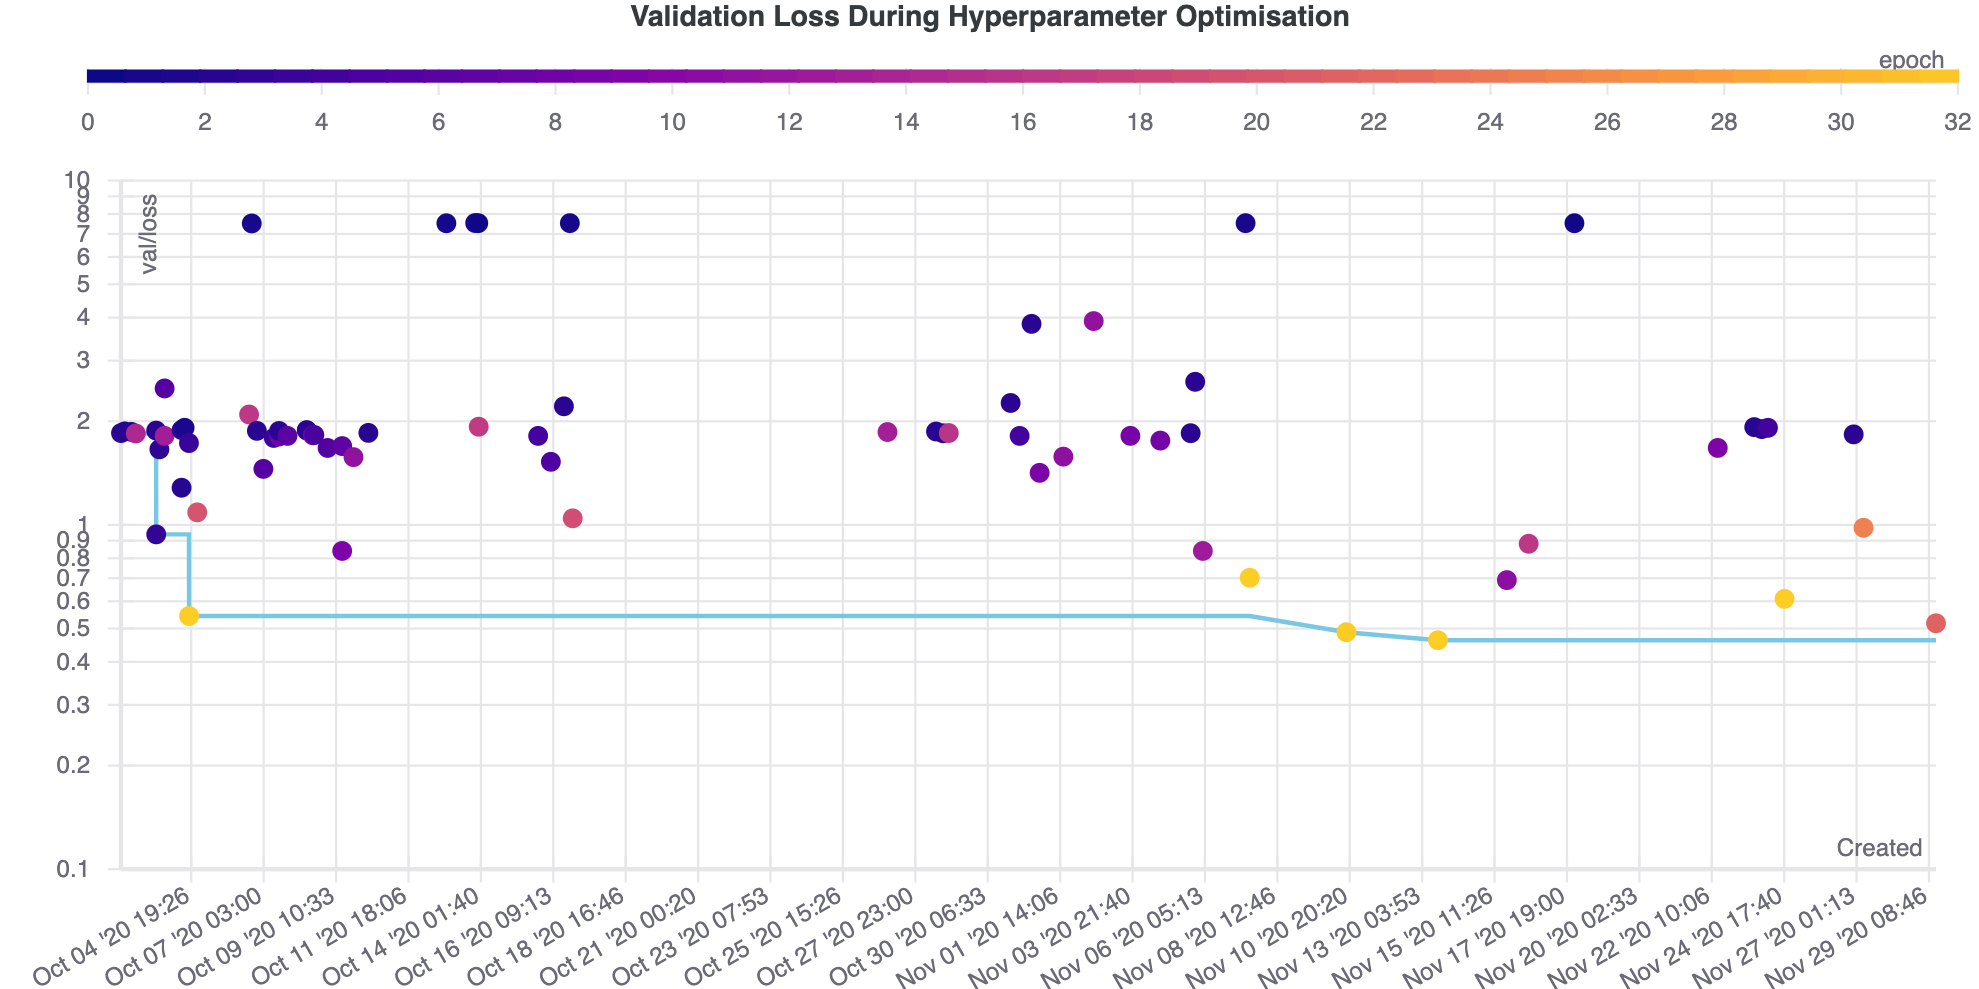
\includegraphics[width=\textwidth]{hyperparameter_optimisation_validation_loss.png}
        \label{fig:hyperparameter_optimisation_validation_loss}
        \caption{Validation loss throughout the hyperparameter optimisation process.}
    \end{subfigure}
    \par\bigskip % force a bit of vertical whitespace
    \par\bigskip
    \begin{subfigure}[b]{\textwidth}
        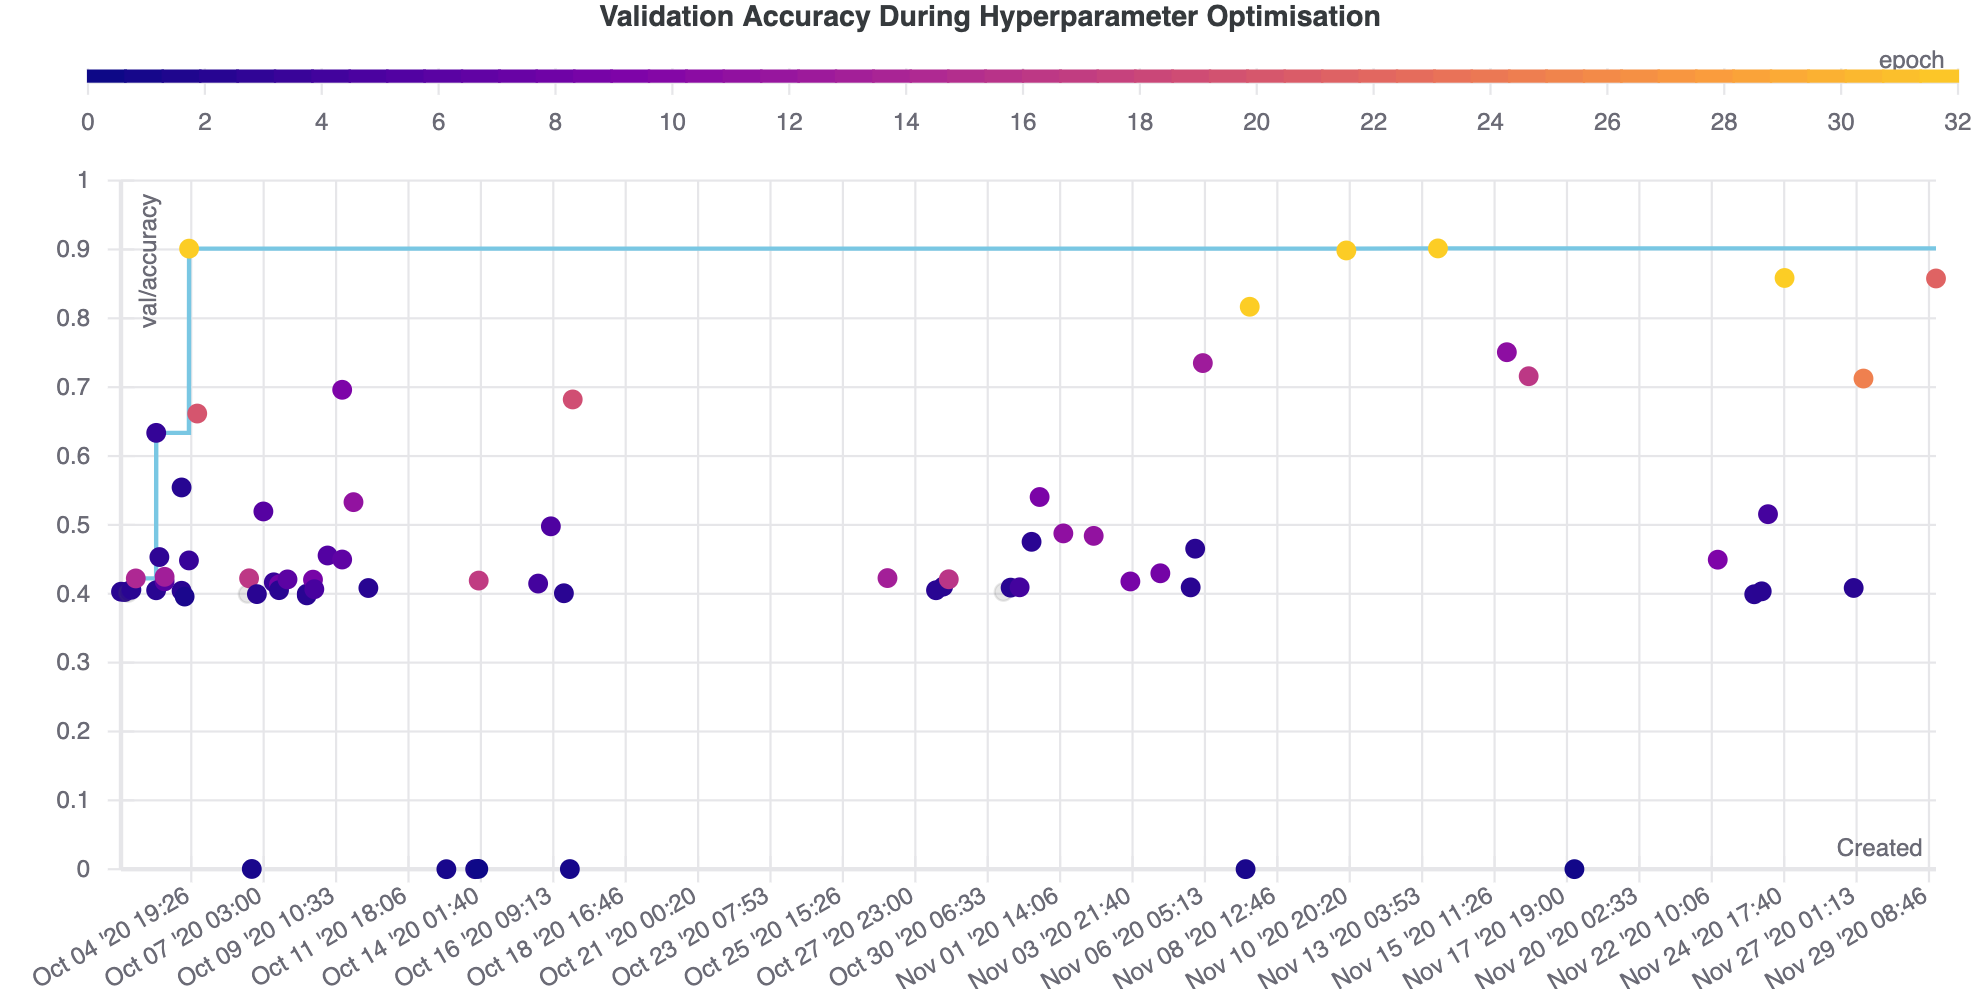
\includegraphics[width=\textwidth]{hyperparameter_optimisation_validation_accuracy.png}
        \label{fig:hyperparameter_optimisation_validation_accuracy}
        \caption{Validation accuracy throughout the hyperparameter optimisation process. Greyed out points correspond to models with a loss greater than 10.}
    \end{subfigure}
    \caption{A summary of validation loss and accuracy throughout the hyperparameter optimisation process. Each point represents a trained model, and its colour indicates how many epochs the model was trained for.}
    \label{fig:hyperparameter_optimisation_validation_loss_and_accuracy}
\end{figure}



\begin{figure}
    \centering
    \begin{subfigure}[l]{0.5\textwidth}
        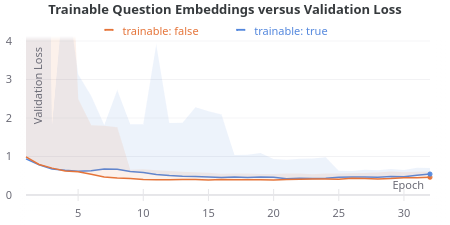
\includegraphics[width=\textwidth]{trainable_question_embedding_validation_loss.png}
        \label{fig:trainable_question_embedding_validation_loss}
        \caption{Validation Loss}
    \end{subfigure}
    \begin{subfigure}[r]{0.49\textwidth}
        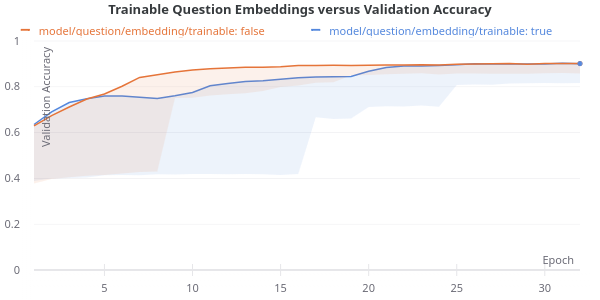
\includegraphics[width=\textwidth]{figures/trainable_question_embedding_validation_accuracy.png}
        \label{fig:hyperparameter_optimisation_validation_accuracy}
        \caption{Validation Accuracy}
    \end{subfigure}
    \caption{}
    \label{fig:hyperparameter_optimisation_validation_loss_and_accuracy}
\end{figure}
 
 
